\section{Valores físicos de los átomos}

Al estudiar los átomos y sus interacciones entre sí hay algunos valores que nos pueden ser de gran utilidad conoce:

\begin{itemize}
    \item Radio atómico
    \item Energía de ionización
    \item Afinidad electrónica
    \item Electronegatividad
\end{itemize}

\subsection{Radio atómico}

\definition{Radio atómico}{Es la mitad de la distancia entre los núcleos de 2 átomos de un mismo elemento que están unidos entre sí.}

Este valor es mayor al final de cada período, de manera que los electrones de los átomos de los elementos que se encuentran más a la derecha de la tabla se encuentran más atraídos por el núcleo, de modo que, como el número de niveles en el que se enlazan los átomos es el mismo, el radio disminuye. Esto se puede ver ejemplificado en la \autoref{fig:tabla_radio_atómico}

\begin{figure}[H]
    \centering
    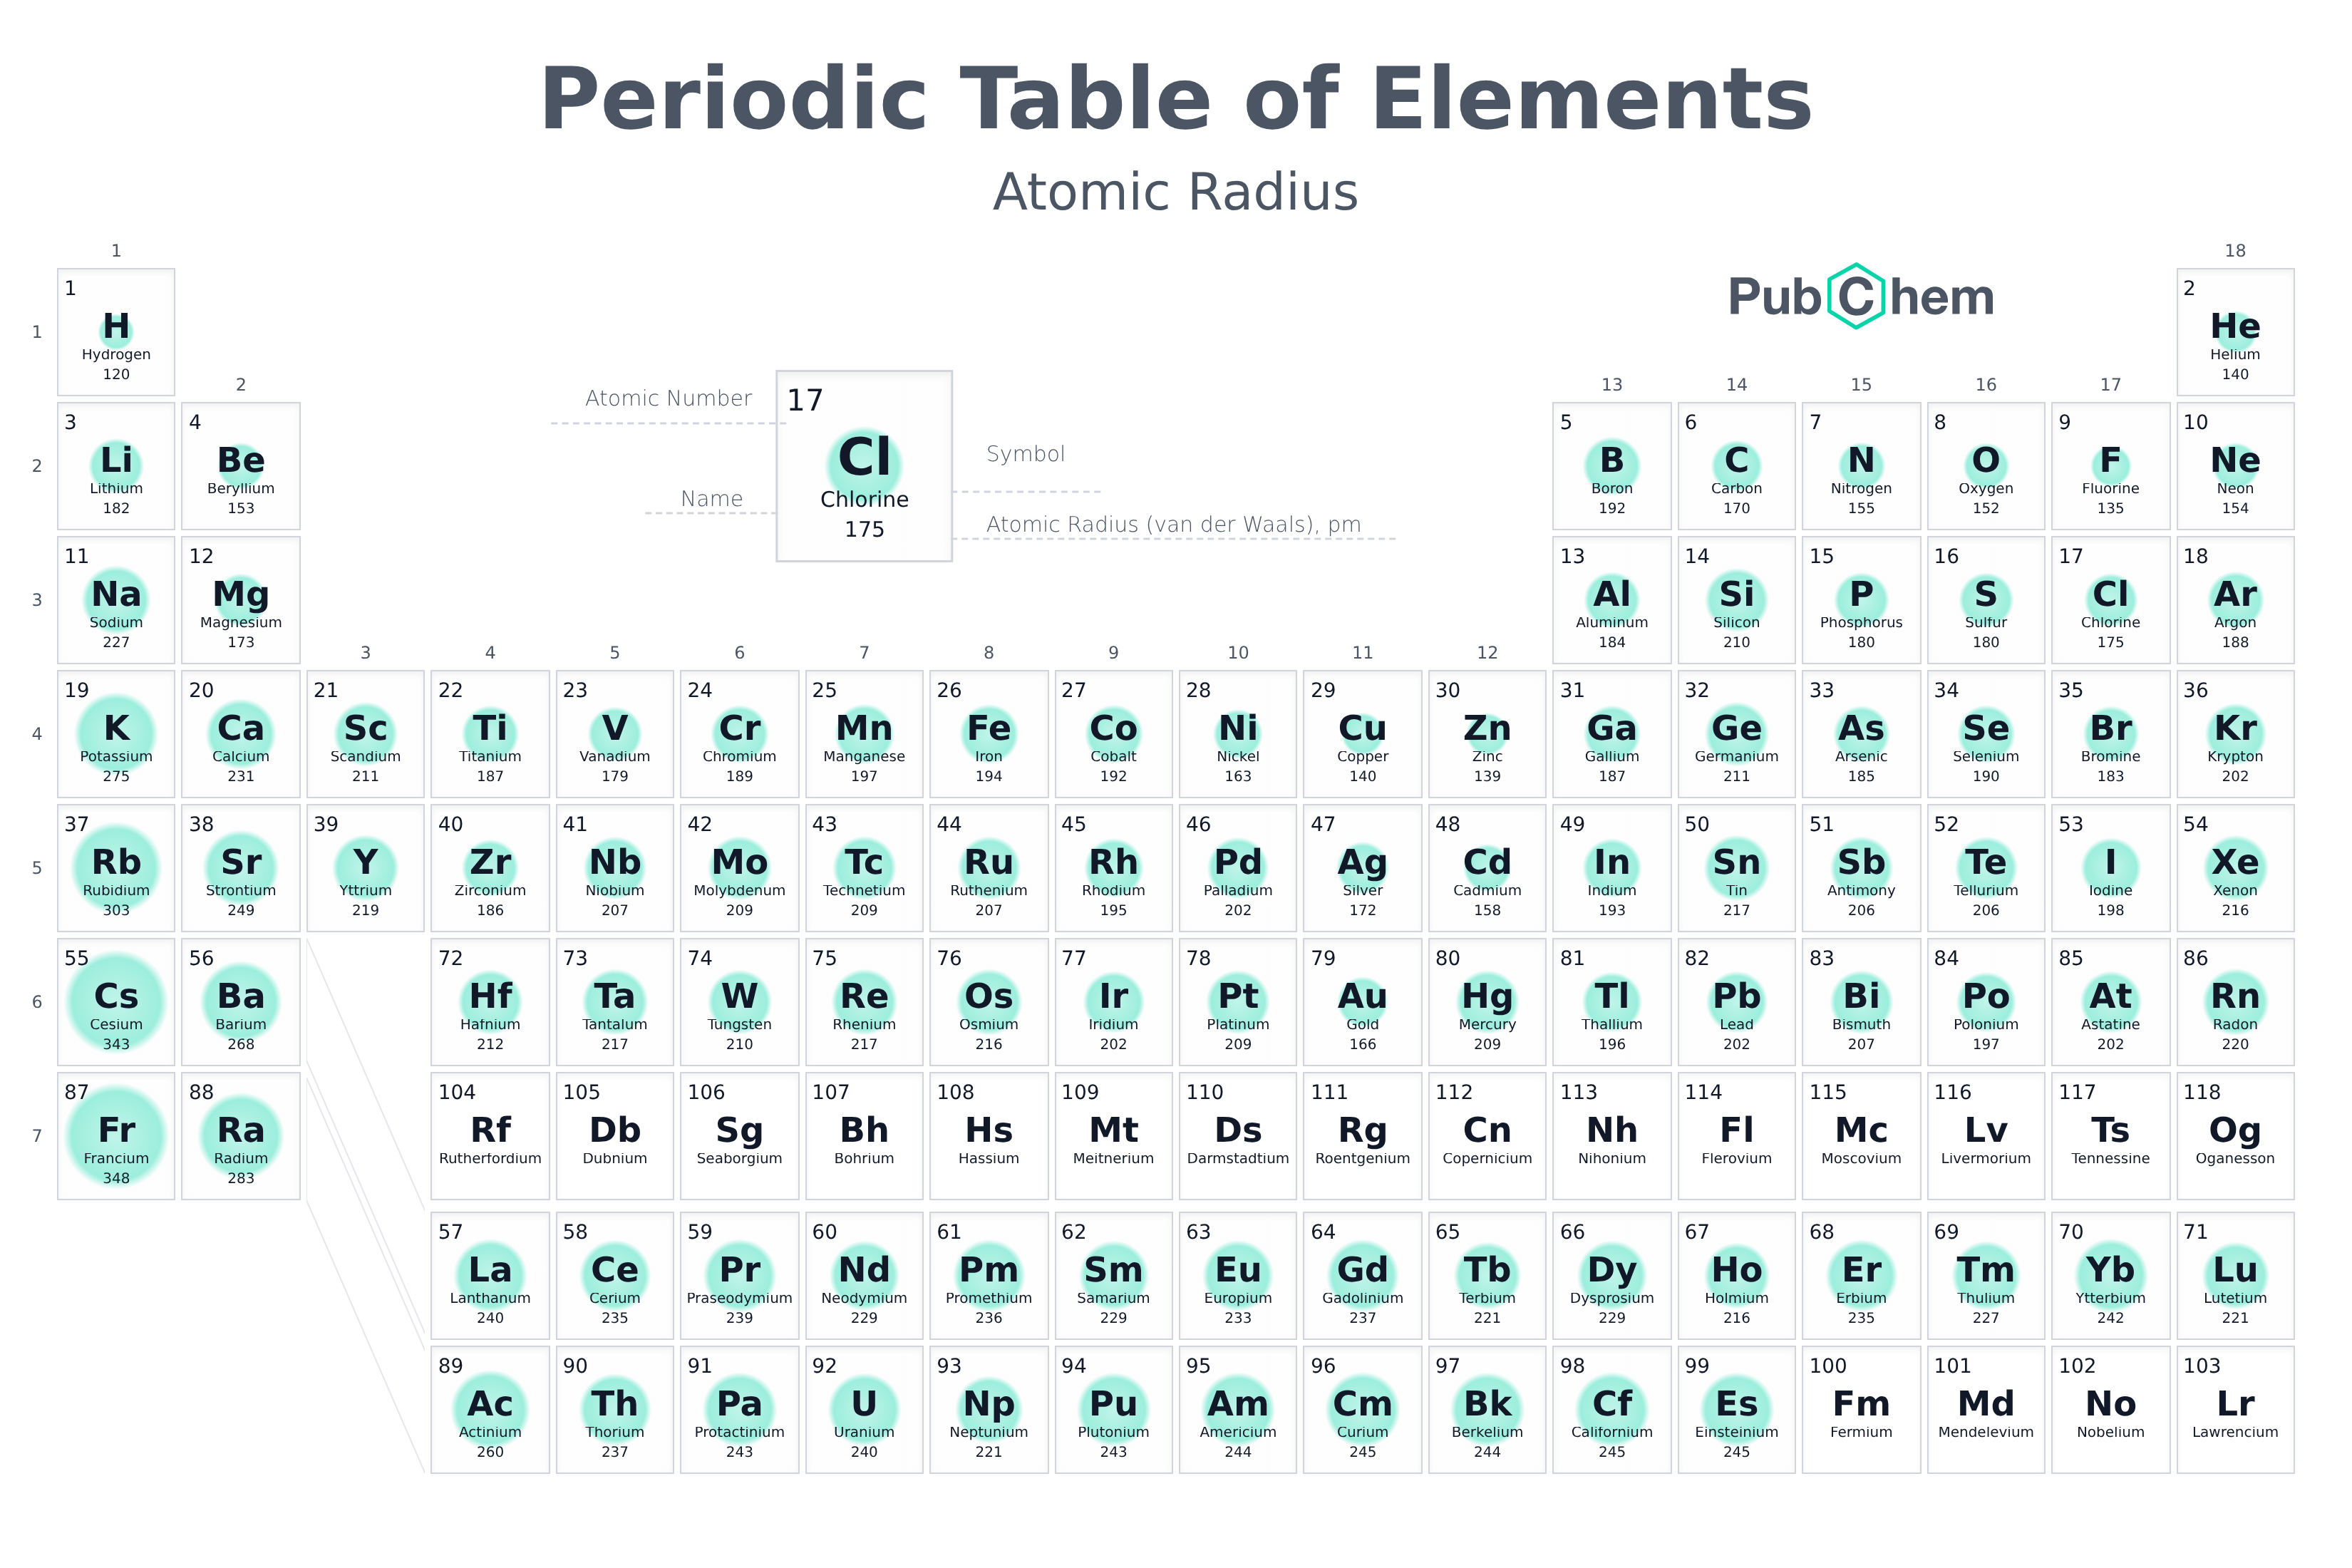
\includegraphics[width=0.9\textwidth]{./images/radio_atómico.png}
    \caption{Tabla periódica con valores de radio atómico para cada elemento. Extraido de PubChem}
    \label{fig:tabla_radio_atómico}
\end{figure}

\subsection{Energía de ionización}

\definition{Energía de ionización}{Mínima energía que hay que suministrar a un átomo neutro y en su estado fundamental, perteneciente a un elemento en estado gaseoso, para arrancarle un electrón.}

La reacción puede expresarse de la siguiente forma:

\begin{equation*}
    A_{(g)}  + E_{1} = A^{+}_{(g)} + 1e^{-}
\end{equation*}

Se expresa en: electrón-voltio ($eV$), julios ($j$) o $\frac{kJ}{mol}$

\begin{figure}[H]
    \centering
    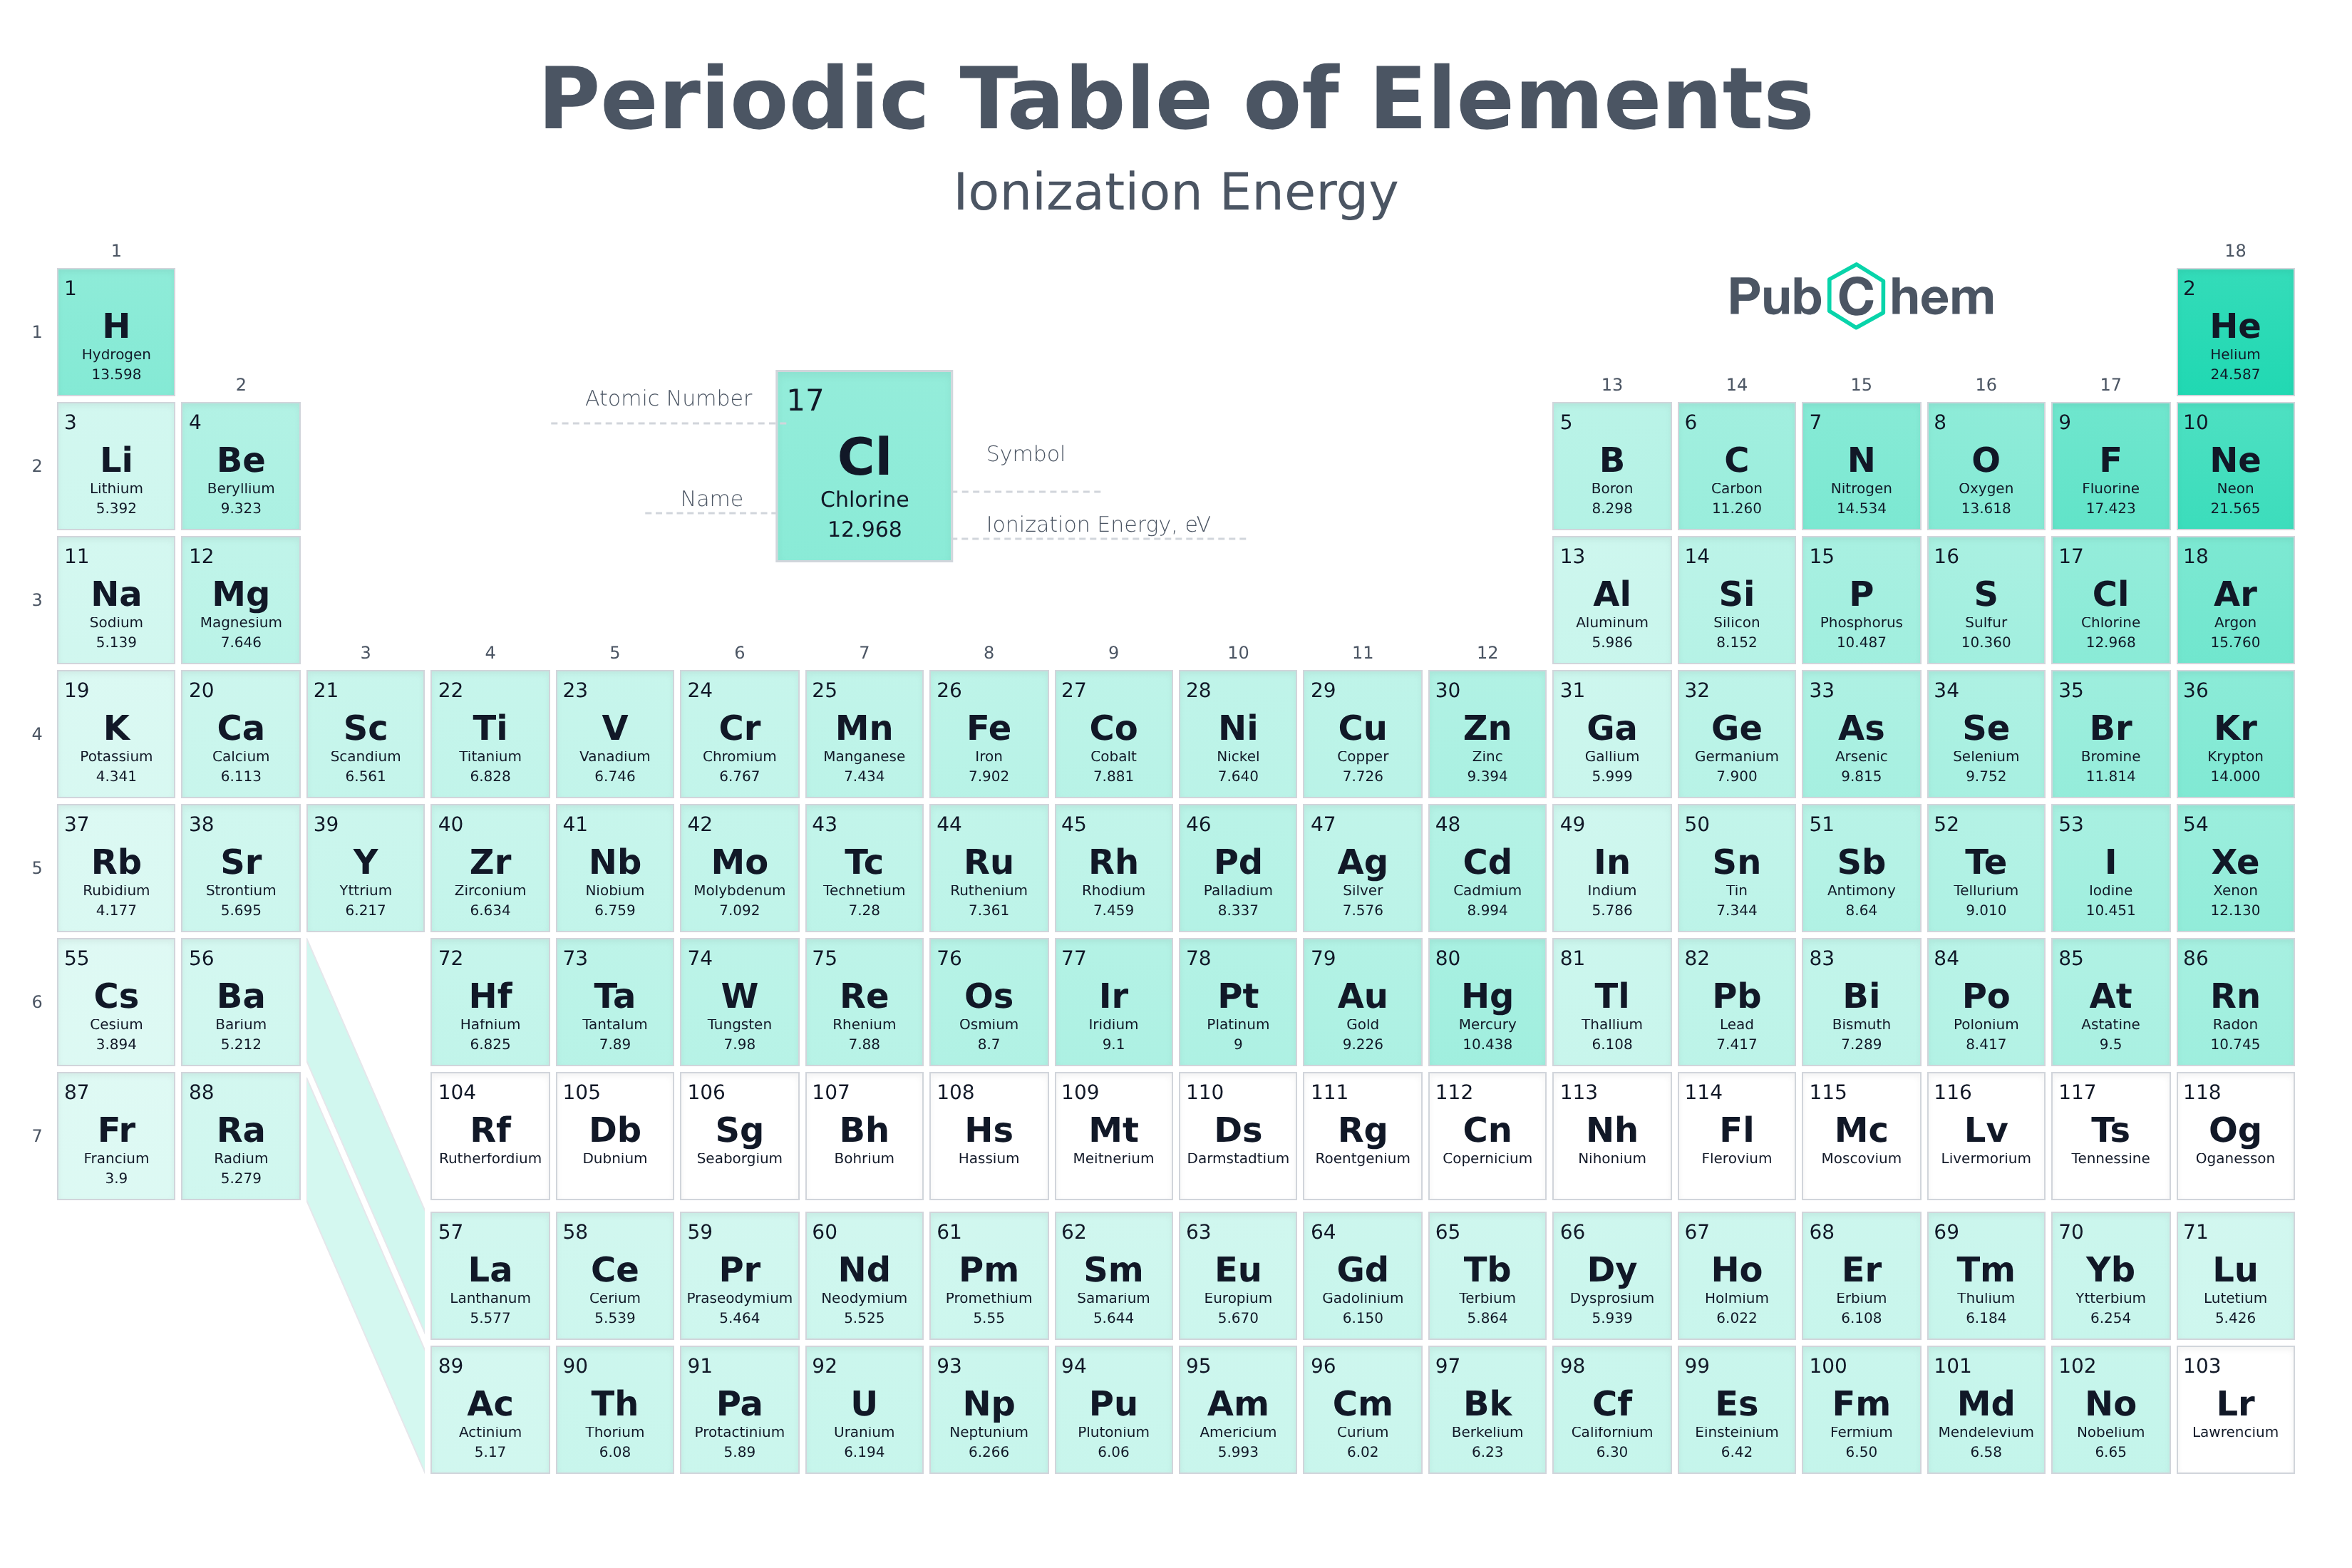
\includegraphics[width=0.9\textwidth]{./images/energía_de_ionización.png}
    \caption{Tabla periódica con valores de energía de ionización para cada elemento. Extraido de PubChem}
    \label{fig:tabla_energía_de_ionización}
\end{figure}

\subsection{Afinidad electrónica}

\definition{Afinidad electrónica}{Cantidad de energía que libera un átomo aislado en fase gaseosa para formar un ion con una carga eléctrica de -1}

Aunque la afinidad electrónica parece variar de forma caótica y desordenada a lo largo de la tabla periódica, se pueden apreciar patrones. Los no metales tienen afinidades electrónicas más bajas que los metales, exceptuando los gases nobles que presentan valores positivos por su estabilidad química, ya que la afinidad electrónica está influenciada por la regla del octeto.
Los elementos del grupo 1, tienden a ganar un electrón y formar aniones -1, completando el subnivel s, mientras que los elementos del grupo 2, que ya lo tienen completo, no presentan esa tendencia. Análogamente sucede en el bloque p, donde las afinidades electrónicas se van haciendo más negativas a medida que nos acercamos a los gases nobles.

\begin{figure}[H]
    \centering
    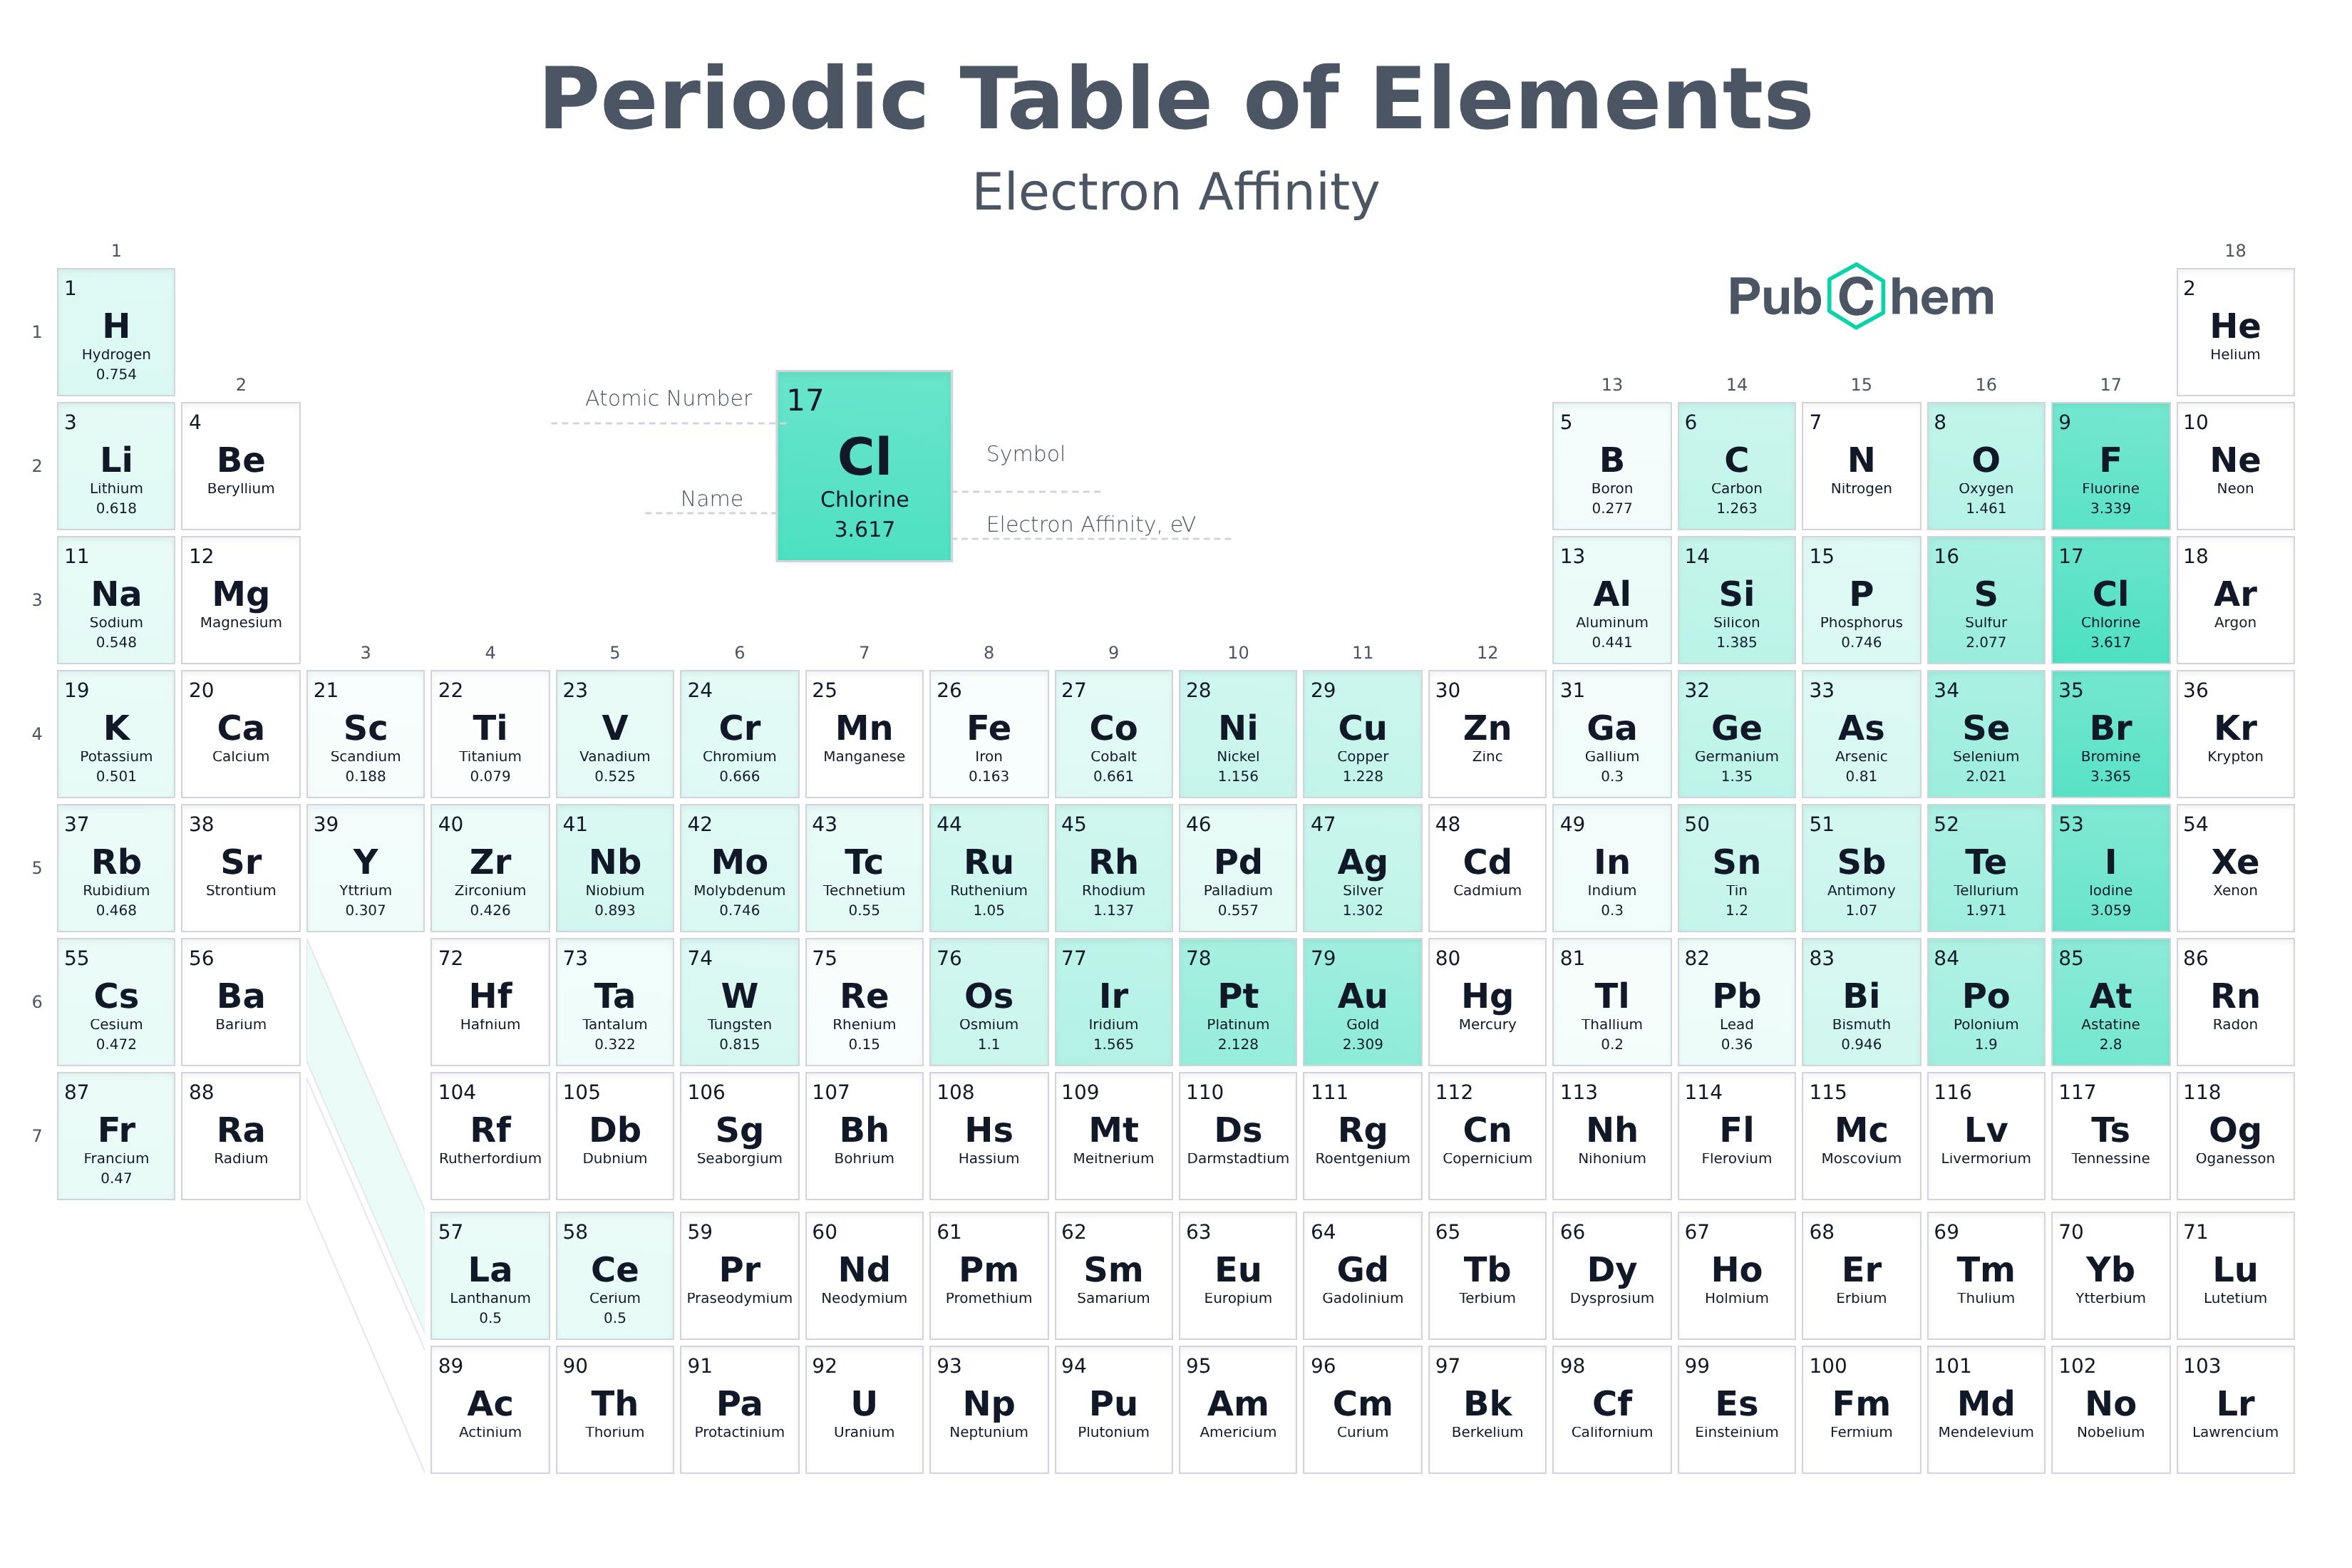
\includegraphics[width=0.9\textwidth]{./images/afinidad_electrónica.png}
    \caption{Tabla periódica con valores de afinidad electrónica para cada elemento. Extraido de PubChem}
    \label{fig:tabla_afinidad_electrónica}
\end{figure}

La afinidad electrónica es de utilidad para saber si un proceso es exotérmico (libera energía) o endotérmico (abosrbe energía).

\begin{align*}
    A_{(g)} + 1e^{-} &= A_{(g)}^{-} + E_{A}
    \\
    \\
    \text{si: } E_{A} > 0 &\Longrightarrow \text{Proceso endotérmico}
    \\
    \text{si: } E_{A} < 0 &\Longrightarrow \text{Proceso exotérmico}
\end{align*}

\subsection{Electronegatividad}

\definition{Electronegatividad}{Es la capacidad de un átomo o grupos funcionales para atraer electrones}

La electronegatividad se mide en la escala de Pauli, la cual va del 0.4 al 4. Conocer la electronegatividad de un átomo es útil para determinar el tipo de enlace que formará tal átomo al unirse a otros y formar moléculas.

\begin{equation*}
    \Delta_{x} = \text{En}_{a} - \text{En}_{b}
\end{equation*}

Valores de electronegatividad:

\begin{itemize}
  \item Covalente no polar:  $\Delta_{x} = 0-0.4$
  \item Covalente polar: $\Delta_{x} = 0.4-1.6$
  \item Iónico: $\Delta_{x} = 1.6-3.3$
\end{itemize}

\begin{figure}[H]
    \centering
    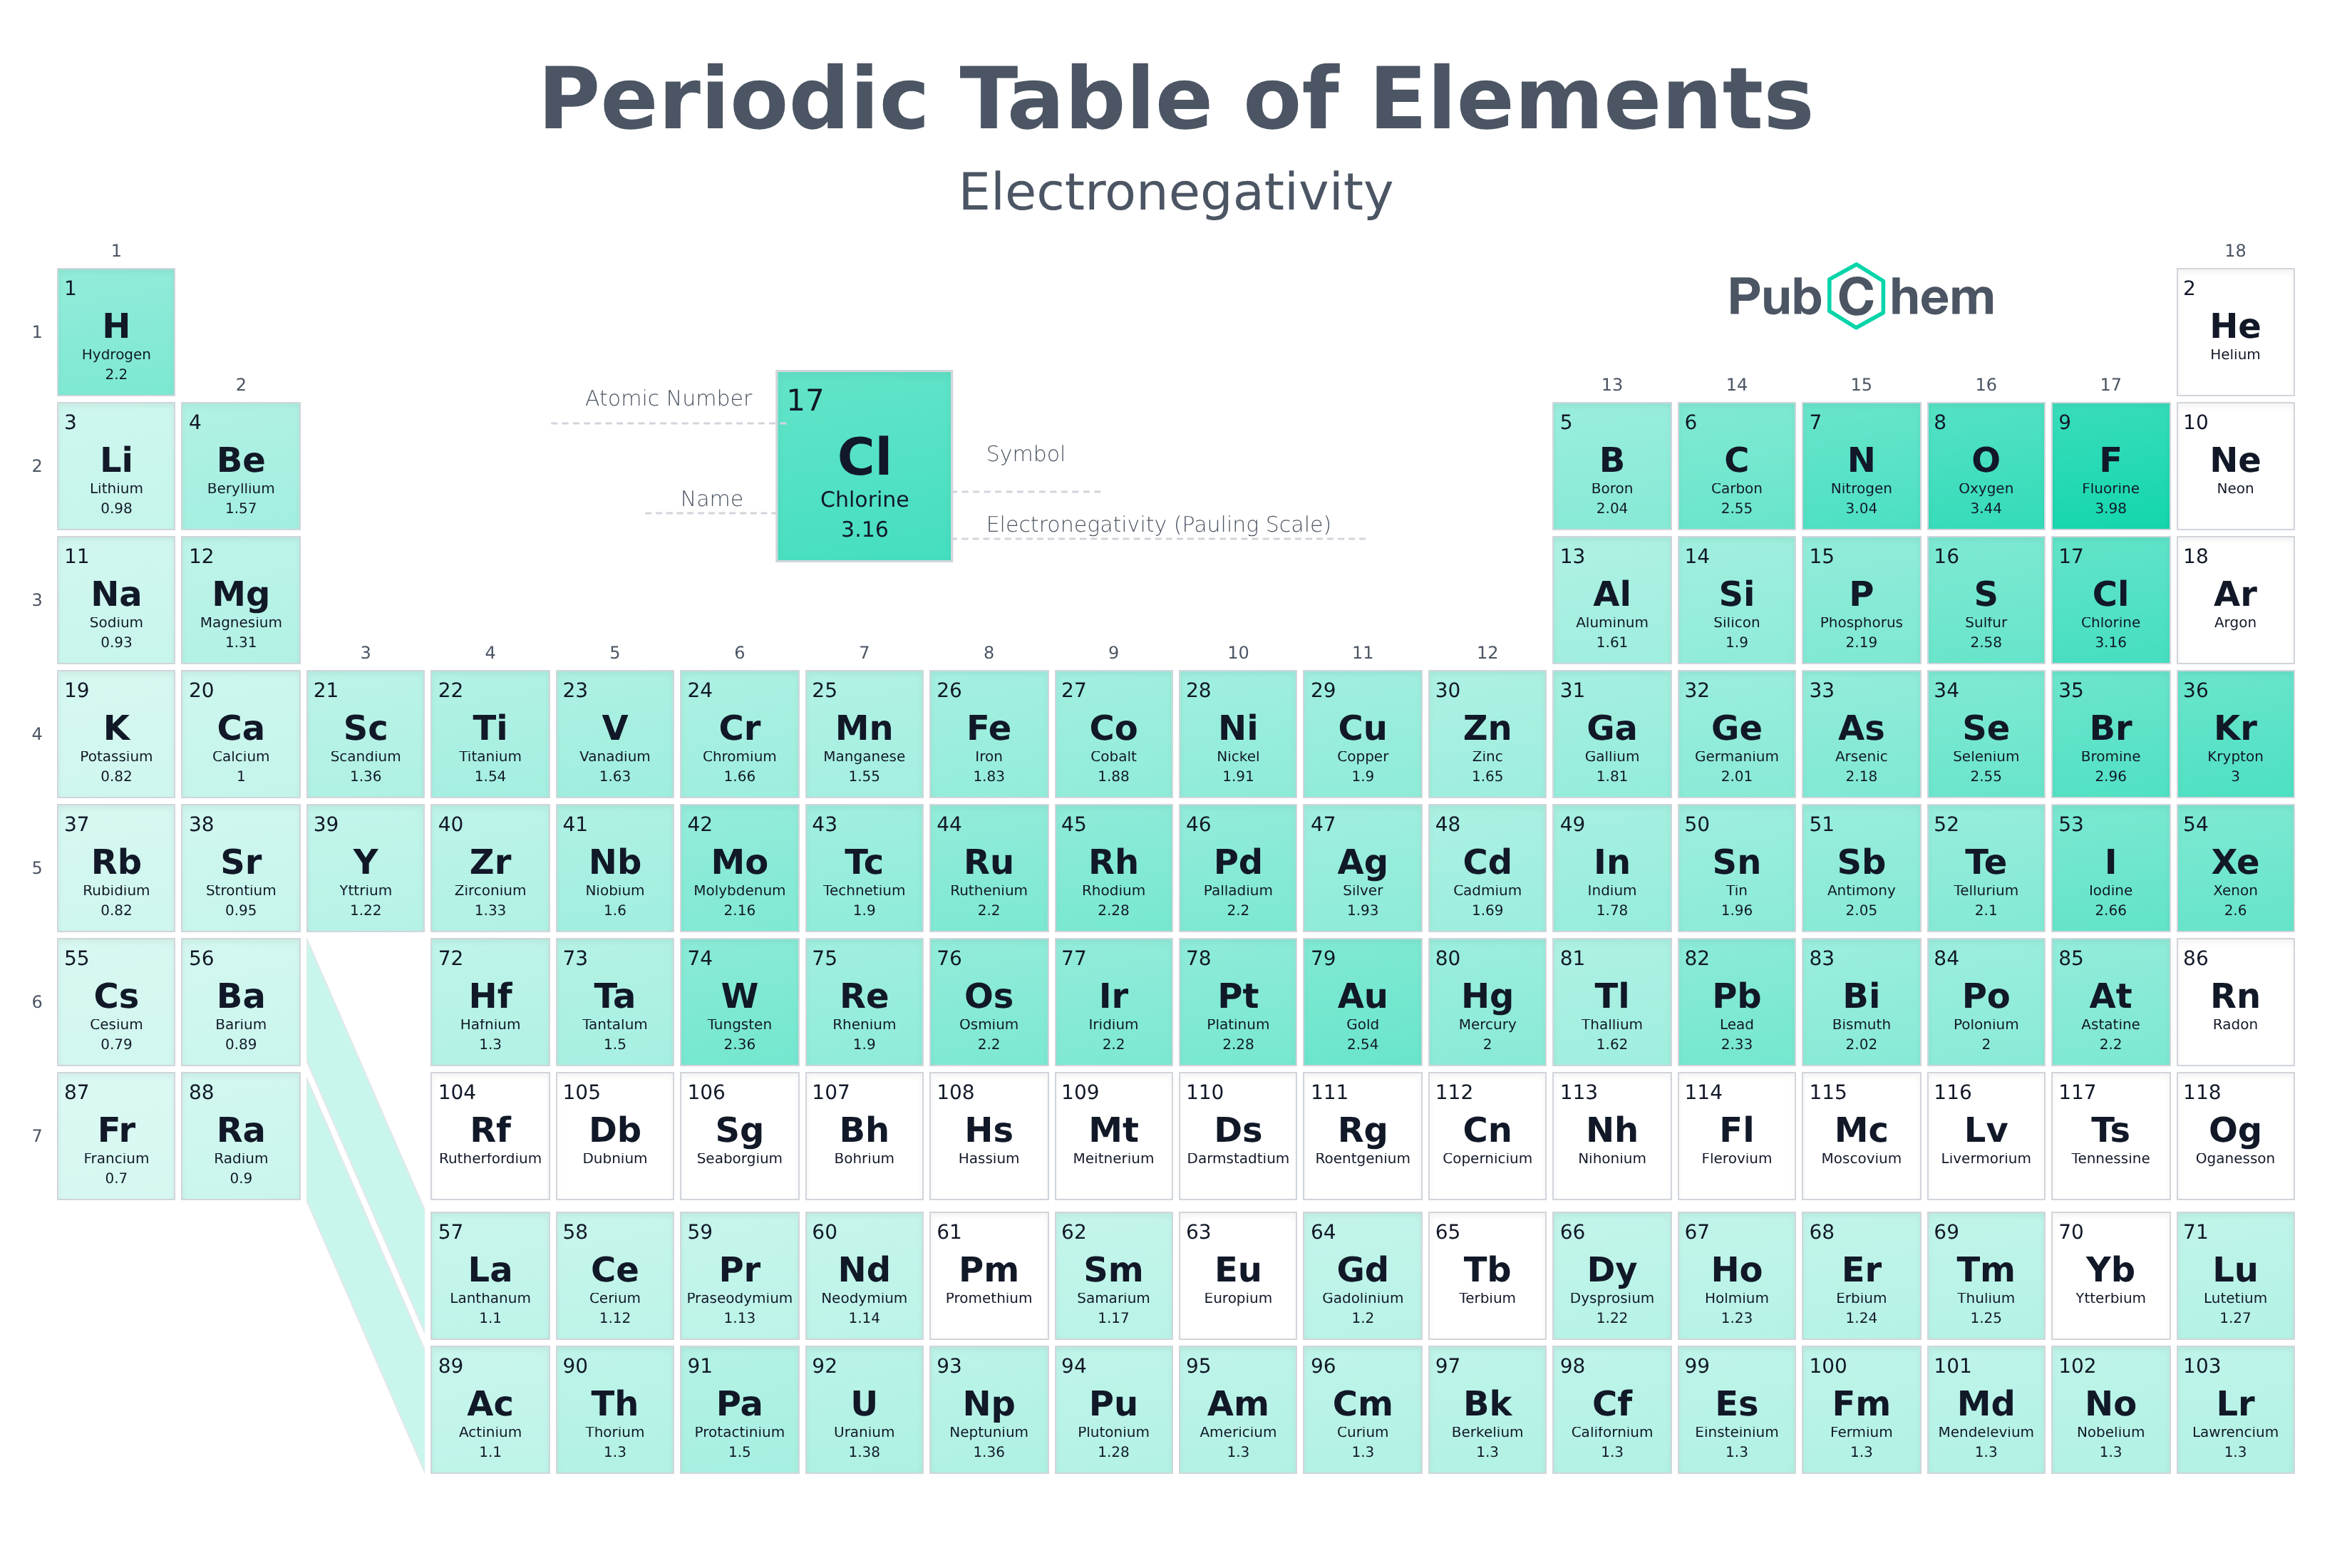
\includegraphics[width=0.9\textwidth]{./images/electronegatividad.png}
    \caption{Tabla periódica con valores de electronegatividad para cada elemento. Extraido de PubChem}
    \label{fig:tabla_electronegatividad}
\end{figure}

\section{Números cuánticos}

Para determinar las características de un átomo dado son útiles los números cuánticos. Estos son una serie de números en los que cada uno de ellos describe una característica del átomo. 

\begin{itemize}
    \item $n$: número cuántico principal
        \begin{itemize}
            \item Marca el nivel de energía del electrón ($e^{-}$)
            \item Describe la distancia relativa al núcleo
            \item Sus valores van del 1 en adelante ($n=1,2,3,...$)
        \end{itemize}
    
    \item $l$: número cuántico azimutal
        \begin{itemize}
            \item Marca el subnivel de energía
            \item Describe la forma del orbital: $s,p,d,f$
            \item Sus valores van del 0 en adelante ($l=0,1,2,3,...$)
            \item Se puede calcular restando 1 al número cuántico principal $n$ ($l=n-1$)
        \end{itemize}
    
    
    \item $m$: número cuántico magnético
        \begin{itemize}
            \item Marca la orientación espacial del orbital
            \item Describe el número de orbitales en un subnivel
            \item Sus valores se definen por el valor de $l$: $m=-l,...,0,...,+l$
    	    \item Ejemplo: Si tenemos $l=1$, tendremos $m=-1,0,+1$, mientras que si tenemos $l=2$ tendremos $m=-2,-1,0,+1,+2$
        \end{itemize}
    
    
    \item $s$: número cuántico del spin
        \begin{itemize}
            \item Describle la orientación en que gira un electrón ($e^{-}$) en un campo magnético
            \item Sus valores pueden ser $-\frac{1}{2}$ ó $+\frac{1}{2}$
        \end{itemize}
    
\end{itemize}

\section{Algunos principios atómicos}

En la física existen ciertos principios que establecen reglas acerca de cómo los átomos y sus componentes deben de comportarse \footnote{O cómo deberían comportarse según los conocimientos humanos de la física.}. El par de principios de la física de partículas que se verán en esta asignatura son los siguientes.

\subsection{Principio de exclusión de Pauli}

Este principio, definido por Wolfgang Ernst Pauli en 1925, dice que: No puede haber dos fermiones en el mismo estado cuántico (esto es, con todos sus números cuánticos idénticos) dentro del mismo sistema cuántico.

\definition{Fermiones}{Son uno de los dos tipos básicos de partículas elementales, y se caracterizan por tener un spin semientero.}

En el caso de los electrones en los átomos, se puede afirmar lo siguiente: Es imposible que dos electrones de un átomo polielectrónico tengan los mismos valores de los cuatro números cuánticos.

Una afirmación más rigurosa sería que: Para los fermiones, la función de onda debe de ser antisimétrica (tener valores opuestos), puesto que de no serlo su valor sería 0.

\subsection{Regla de Hund}

Es un principio físico compuesto de 3 reglas formulado por Friedrich Hund en 1927. El enunciado principal es:

\definition{Regla de Hund}{“Al llenar orbitales de igual energía (los tres orbitales p, los cinco d, o los siete f) los electrones se distribuyen, siempre que sea posible, con sus espines paralelos, llenando los orbitales con la multiplicidad mayor. La configuración atómica es más estable (es decir, tiene menos energía) cuanto más electrones desapareados (espines paralelos) posee.”}

Las 3 reglas particulares mencionadas anteriormente son:

\begin{enumerate}
    \item Para una configuración electrónica dada, el término de menor energía es aquel que tenga el mayor espín total ($S_{t}$);
    \item Para un espín total dado, el término de más baja energía es aquel que tiene el número L más grande;
    \item Para un término de espectroscopia dado:
        \begin{itemize}
            \item En un átomo teniendo su capa externa medio llena o menos,
            \item El nivel de menor energía será el que tenga el menor número $J$ posible.
            \item En un átomo que tenga su capa externa más que medio llena
            \item El nivel de menor energía es aquel que tenga el mayor número $J$ posible.
        \end{itemize}
\end{enumerate}

Así pues:

\begin{itemize}
    \item Todos los orbitales deben estar tener electrones en paralelo (en un estado apareable) antes de que un orbital gane un segundo electrón.
    \item Cuando un orbital gana un segundo electrón, éste deberá estar apareado con el primero (espines opuestos o antiparalelos).
\end{itemize}